%%%%%%%%%%%%%%%%%%%%%%%%%%%%%%%%%%%%%%%%%%%%%%%%%%%%%%%%%%%%%%%%%%
\section{Análisis de los conjuntos de datos}
\label{sec:sustdata}

En ámbitos como el Procesado de Lenguaje Natural (del inglés \gls{nlp}) o el reconocimiento facial, la disponibilidad de numerosas fuentes de datos ha sido imprescindible para acelerar el desarrollo de técnicas de minería de datos y de aprendizaje automático (\gls{ml}).

\vspace{3mm}

A diferencia de estos campos, el contexto energético experimenta un menor grado de disponiblidad de datasets. La protección de la privacidad de los usuarios en el proceso de medición y análisis de su comportamiento energético supone que exista un menor número de datasets públicos enfocados a implementaciones reales. No obstante, la búsqueda de la optimización de la distribución energética y de la reducción del consumo de los usuarios, aparte de otras motivaciones ambientales, ha instado en los últimos años a múltiples ingenieros y científicos a lo largo del mundo a crear datasets públicos enfocados a la investigación (ver Tabla \ref{tab:datasets}). 

\vspace{3mm}

En este contexto han cobrado gran importancia las técnicas de Monitorización de Cargas no Intrusiva (del inglés \gls{nilm}). Como se ha introducido en la Sección \ref{sec:ioe}, cada vez se produce una mayor integración de las tecnologías de \gls{ioe} en el ámbito de las \gls{sg}s para obtener una mayor monitorización del comportamiento energético en los hogares. Es por ello que el fin principal de las técnicas de \gls{nilm} reside en establecer una desagregación energética para poder estimar de una forma precisa el consumo individual de cada uno de los dispositivos y electrodomésticos que hay en una vivienda. Para ello, se instalan medidores en cada circuito y después, se analizan, tanto a nivel interno como a nivel externo de la vivienda, los cambios de los parámetros eléctricos en cada instante temporal.~\cite{nilm} \cite{greend}

\vspace{3mm}

Teniendo esto en cuenta, se puede expresar que las técnicas de \gls{nilm} se caracterizan por su bajo coste y por su facilidad y flexibilidad de despliegue. No obstante, el proceso de medición y recolección de datos puede llegar a requerir mucho tiempo y esfuerzo. Por ello, en el contexto de la investigación es importante que los datos tengan una disponibilidad pública para progresar en el desarrollo de técnicas de minería de datos y de aprendizaje automático en el ámbito energético. 

\vspace{3mm}

En la Tabla \ref{tab:datasets} se exponen los múltiples datasets residenciales que han sido estudiados en esta fase de diseño, junto con información relativa a la implementación real sobre la que se ha basado cada uno de ellos, como es la ubicación de la misma, el número de viviendas total, el lapso temporal que comprende el despliegue, la frecuencia de las muestras tomadas y los parámetros eléctricos medidos. En virtud de las motivaciones y objetivos del presente \gls{tfm}, es importante tener en cuenta ciertos requisitos para evaluar los conjuntos de datos disponibles y seleccionar el más apropiado:

\vspace{1mm}

\begin{itemize}
    \item Cantidad: En primera instancia, es imprescindible revisar la cantidad de datos que aporta cada conjunto. En otros términos, para llevar a cabo un análisis estadístico del comportamiento energético de una ubicación se requiere partir de un conjunto de datos que agrupe las mediciones de un gran número de edificios residenciales. Adicionalmente, este análisis debe comprender extensos períodos temporales de medición para visualizar de forma correcta el comportamiento de los usuarios y predecir patrones de consumo a lo largo del tiempo.
    \item Calidad: Se debe evaluar la calidad de los datos recogidos, la cual responde en parte con la resolución de las medidas que se toman. Como se puede observar en la Tabla \ref{tab:datasets}, algunos datasets como \textit{REDD} y \textit{BLUED} se centran en monitorizar los edificios residenciales a una frecuencia de muestreo alta. En el contexto de las tecnologías de \gls{nilm}, esto aporta una vista más representativa del comportamiento energético a nivel interno en una vivienda y permite una desagregación energética más precisa. Por lo tanto, cuanto mayor sea la frecuencia de adquisición de medidas, mayor será la resolucion de los datos. 
    
    \clearpage

    \item Ubicación: En términos de la ubicación de la implementación real sobre la que se han adquirido las mediciones, es de importancia conocer a la hora de analizar los datos las diferencias de voltaje que se manejan en cada país. Por ejemplo, en el caso de datasets como \textit{BLUED} o \textit{Smart*}, los cuales provienen de ciudades de Estados Unidos, trabajarán a tensiones menores de 120V, mientras que otros como \textit{ECO} o \textit{GREEND}, cuyos datos se han adquirido en países europeos, lo harán con tensiones de hasta 230V. \cite{greend}
    \item Parametrización: Por lo general, un dataset dedicado a las tecnologías de \gls{nilm} estará constituido por una colección de muestras de voltaje (V), corriente (I) y potencia activa (P), reactiva (Q) y aparente (S). Cada una de estas muestras vendrá asociada a una marca de tiempo y a un identificador que haga referencia a la vivienda o medidores a los que corresponde. Adicionalmente, algunos de los datasets que se exponen en la Tabla \ref{tab:datasets}, como son \textit{HUE} o \textit{SustDataED}, también incluyen información relativa a parámetros ambientales. Esto, sobre todo en el contexto de las \gls{sg}s, proporciona información fundamental sobre el impacto de las condiciones climáticas en el comportamiento de los usuarios.
    \item Generación fotovoltaica: Considerando el contexto de \gls{sg}s en el que se engloba este \gls{tfm}, es de vital importancia seleccionar un conjunto de datos que aporte información relativa a la generación de energía a través de fuentes renovables, como ocurre en el caso de \textit{Smart*} o \textit{SustDataED}. En relación con esto, se expondrá en la Sección \ref{sec:global} el estudio de una plataforma específica dedicada a la adquisición de datos de generación energética.
\end{itemize}

\begin{sidewaystable}
    \centering 
    \begin{tabularx}{\textheight}{|X|X|X|X|X|X|}
        \hline
        \rowcolor[HTML]{EFEFEF} 
        Nombre & Localización & Nº de residencias & Período de medición (días) & Resolución de medición & Parámetros \\ \hline
        \textit{BLUED} \cite{blued} & Pittsburg (Estados Unidos) & 1 & 8 & 12KHz &  I, V, eventos de switch \\ \hline
        \textit{ECO} \cite{eco} & Thun (Suiza) & 6 & 244 & 1Hz & P \\ \hline
        \textit{GREEND} \cite{greend} & Italia y Austria & 9 & 310 & 1Hz & P \\ \hline
        \textit{HUE} \cite{hue} & British Columbia, Canada & 28 & 60 & 1Hz & P \\ \hline
        \textit{iAWE} \cite{iawe} & Nueva Delhi (La India) & 1 & 73 & 1Hz & V, I, P, S \\ \hline
        \textit{REDD} \cite{redd} & Boston (Estados Unidos) & 6 & 19 & 15KHz & V, P \\ \hline
        \textit{Smart*} \cite{smart*} & Massachussets (Estados Unidos) & 3 & 90 & 1min & P, S, V, I \\ \hline
        \textit{SustDataED} \cite{sustdata} & Madeira (Portugal) & 50 & 504 & 1min & I, V, P, Q \\ \hline
        \textit{UK-DALE} \cite{ukdale} & Reino Unido & 5 & 499 & 16KHz & P, estado de switch \\ \hline
    \end{tabularx}
    \caption{Comparación entre datasets públicos en el ámbito \acrshort{nilm} \cite{greend} \cite{intrusive} \cite{tabladatasets}}
    \label{tab:datasets}
\end{sidewaystable}

Como se ha introducido en el Capítulo \ref{ch:intro}, el objetivo principal que se prentende con este \gls{tfm} es desarrollar técnicas de \gls{ml} para identificar y predecir de forma precisa los errores que se pueden producir en una \gls{sg} durante el proceso de distribución energética. A partir de ello, se expresa la necesidad de seleccionar un conjunto de datos en el que se pueda analizar el comportamiento de múltiples usuarios, tanto de consumo como de producción, durante un extenso período de tiempo. 

\vspace{3mm}

De igual manera, es importante que las muestras tengan una buena resolución y que proporcione información en cada instante sobre las condiciones climáticas de la ubicación donde se encuentran las viviendas. Bajo las premisas anteriores, se ha finalizado el proceso de estudio y análisis de los diferentes conjuntos de datos llegando a la conclusión de que el dataset más adecuado a emplear en este \gls{tfm} es \textit{SustDataED}.

\clearpage

\subsection{\textit{SustDataED}}

El dataset \textit{SustDataED} \cite{sustdata} es creado a partir del proyecto de investigación \gls{sinais}, dedicado al diseño, implementación y despliegue de sistemas \gls{nilm} de bajo coste. Surge con el objetivo de proporcionar una retroalimentación ecológica a los usuarios para fomentar un comportamiento energético sostenible y un mayor uso de las fuentes de energía renovables.

\vspace{3mm}

El dataset \textit{SustDataED} engloba cinco años de datos de consumo y producción energética de 50 hogares de la ciudad de Funchal (Madeira, Portugal)con una resolución o frecuencia de adquisición de nuevas muestras por minuto. Debido a esto, se caracteriza por comprender una gran cantidad de información eléctrica que tendrá que ser posteriormente procesada de forma exhaustiva (ver Sección~\ref{sec:preprocesado}).

\vspace{3mm}

Pese a la necesidad de procesamiento que conlleva, el uso de \textit{SustDataED} en el presente \gls{tfm} brinda ciertas ventajas. Entre otras, aporta un gran perspectiva del comportamiento eléctrico a largo plazo de múltiples hogares con diferentes características y ofrece un enfoque medioambiental, ya que mediante la adquisición de los datos relativos a las condiciones climáticas posibilita el análisis de la correlación de las mismas con el consumo y la producción de energía de los usuarios.

\subsection{Estructura del dataset}

El proceso de creación del dataset y la adquisición de los datos del mismo se divide en cuatro despliegues diferentes. 

\begin{figure}[h!]
    \centering
    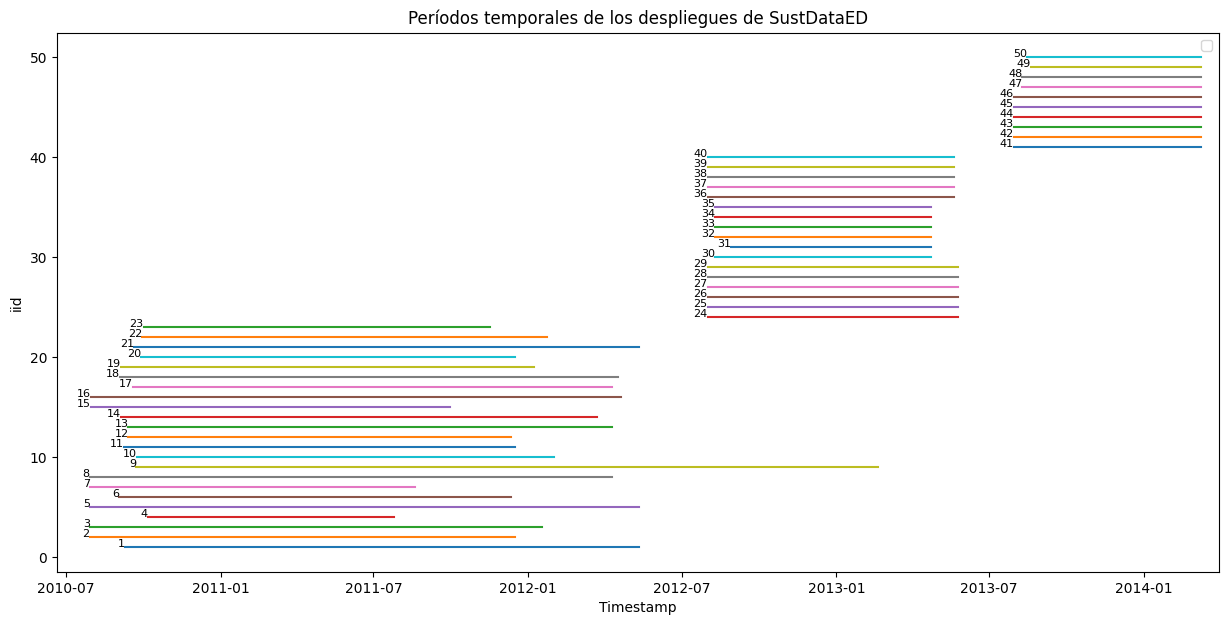
\includegraphics[width=1\textwidth]{img/diseno/despliegues.png}
    \caption{Representación del período temporal que comprende el proceso de recolección de datos para cada hogar}
    \label{fig:bigdata2}
\end{figure}


\subsection{Global Solar Atlas}
\label{sec:global}


%/cite hue
%Consumption history data, simulated solar data, and weather data is stored in simple commaseparated-value (CSV) files. The summary data is stored in a fixed-length format to may it easy to
%read. There are a total of 27 files in this dataset. Table 1 describes the files within the dataset. Data
%frequency for all files is hourly (in local Pacific timezone). Data was downloaded from BCHydro's
%customer web porthole by each customer who then donated the data for research. Weather data was
%downloaded from the nearest Environment Canada [5] weather station. Simulated solar data was
%generated by a tool provided by the US Department of Energy [4].




























%hacer intro en relacion con el apartado de big data

%%para intro -->

%cite stab

%There are two main types of renewable energy data: geospatial and
% temporal data. Geospatial data is concerned with the locations, while
% temporal data is concerned with data time characteristics. For renewable energy, Geospatial data may include the location of transmission
% infrastructure, cities, factories, hospitals, schools, roads, etc. (Shekhar
% et al., 2012); this data is based mainly on Geographical Information Systems (GIS) tools. Temporal data may include the consumption patterns
% with respect to time (annually, monthly, weekly, daily, and hourly)
% besides the amount of energy (e.g., sunshine) during different times
% of day or year.
% A third type user classification data can be the social classification,
% users can be classified into categories not only according to geographic
% areas but also to their social stratums that can be an indicator for daily
% consumption curves (Zhou et al., 2016a). The weather data (e.g., angle
% of the sun rays, wind speed and direction, temperature, pressure, cloud
% cover, humidity, etc.) play a basic role in decision-making support in
% power stations (Zhou et al., 2016b). Hence, the integration between
% supply and demand data, spatial data, and temporal data can support
% strategic decisions such as location selection for renewable energy
% stations to improve output, productivity and efficiency. For a comprehensive review on big data and its techniques for energy systems, the
% reader is referred to the works by Jiang et al. (2016), Molina-Solana
% et al. (2017), Ma et al. (2017).